\section{Related Work}
\label{sec:related}





\paragraph{Towards Universal 3D Reconstruction.}

In contrast to the traditional approach of designing specialized methods for distinct reconstruction tasks, recent efforts have shown great promise in solving them jointly with a single feed-forward architecture.
Early works like DeMoN \cite{UmmenZUMIDB2017}, DeepTAM \cite{ZhouUB2020} or DeepV2D \cite{TeedD2020} explored this direction with CNNs but did not match the performance of classical expert models.
Enabled by advances in deep learning, recent methods like PF-LRM \cite{WangTBXLSWXZ2024}, RayDiffusion \cite{ZhangLKYRT2024}, DUSt3R \cite{WangLCCR2024}, VGGSfM \cite{WangKRN2024}, and VGGT \cite{WangCKVRN2025} scale up transformers on large amounts of data.
Despite this breakthrough, these methods are still limited to
a subset of 3D reconstruction tasks with fixed inputs and output modalities, %
a small or fixed number of views, or they only work well in relatively constrained, typically object-centric, scenarios.
With \coolname, we overcome these limitations by designing a geometrically grounded and flexible architecture that supports heterogeneous input and output modalities for any number of input views.



\begin{figure*}[!t]
\centering
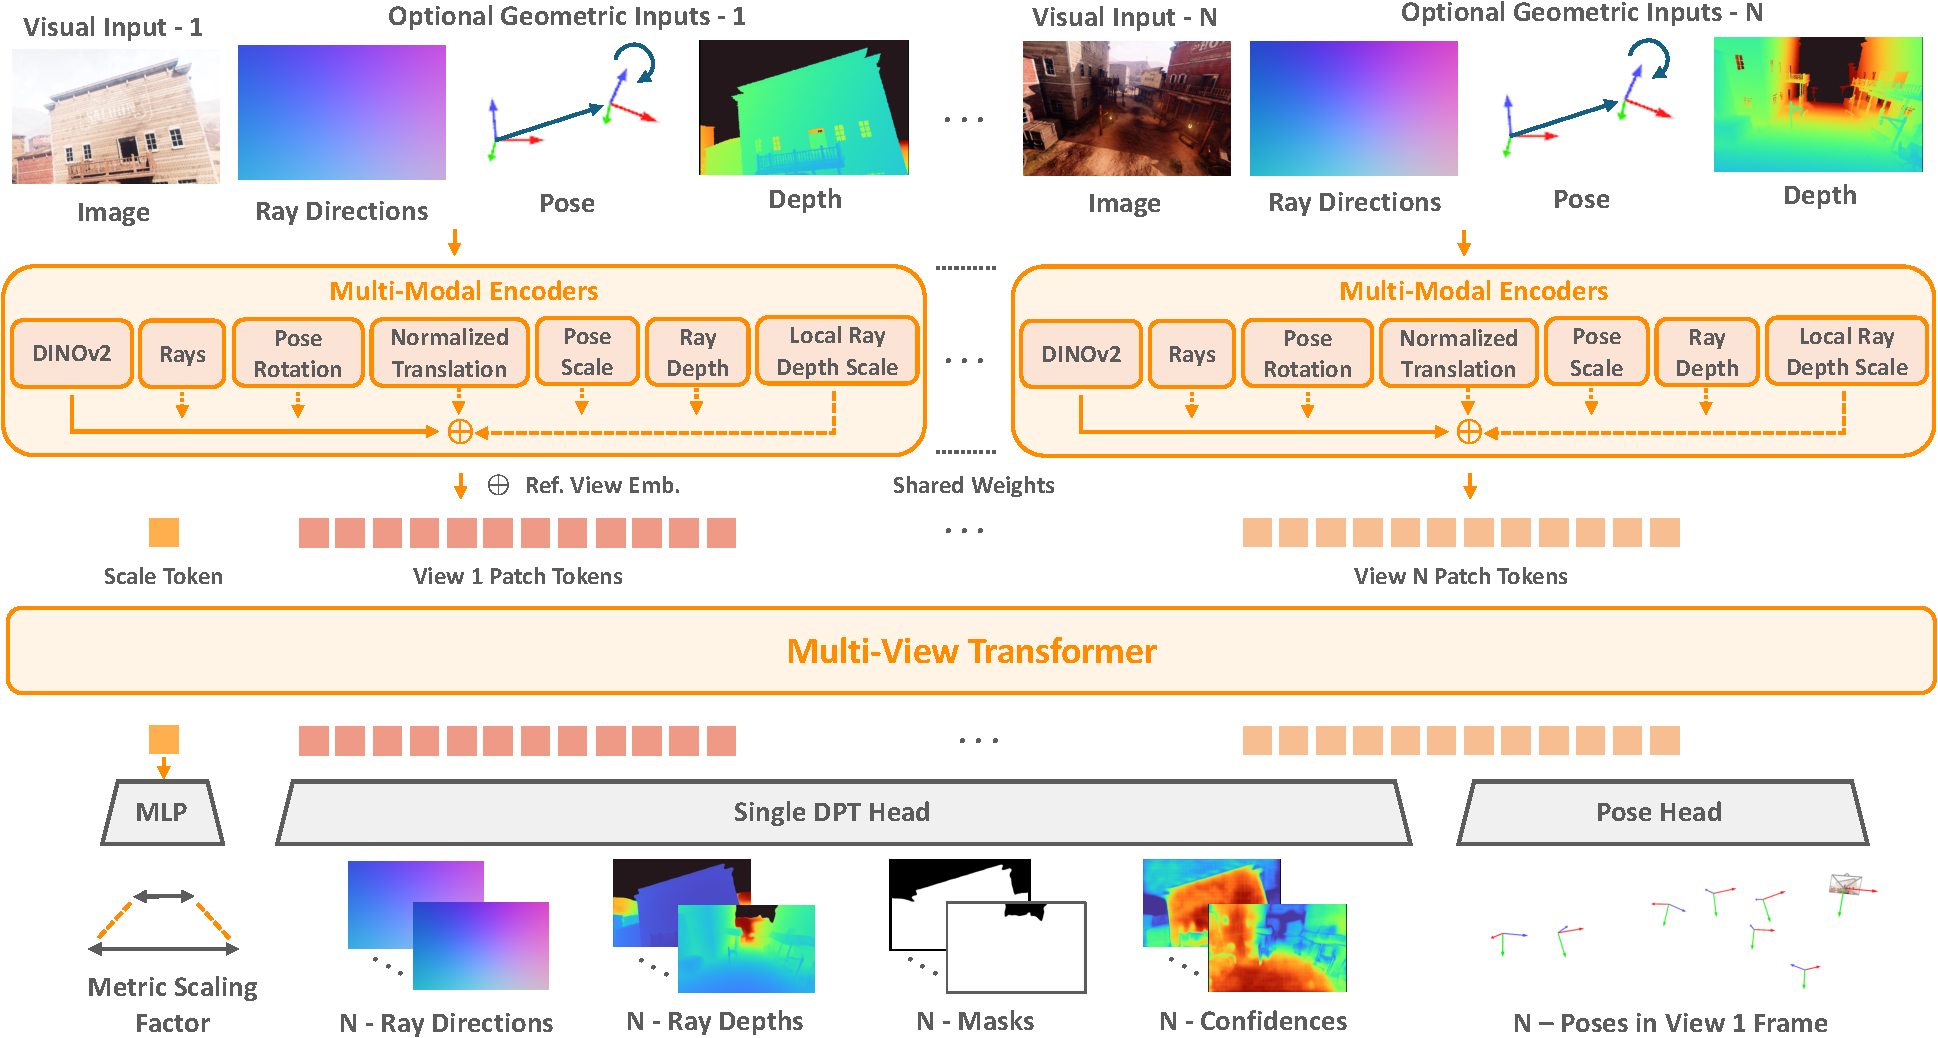
\includegraphics[width=0.9\textwidth]{figs/MapAnything_Method.pdf}
\caption{\label{fig:method}%
\textbf{Overview of the \coolname Architecture.}
Given $N$ visual and optional geometric inputs, the model first encodes the images and the factored representation of the geometric inputs into a common latent space where the patch features (for images, rays \& depth) and broadcasted global features (for translation, rotation, pose scale across all pose inputs \& depth scale local to each frame) are summed together.
Then, a fixed reference view embedding is added to the first view's features and a single learnable scale token is appended to the set of $N$ view patch tokens.
These tokens are then input into an alternating-attention transformer.
We use a single DPT to decode the $N$ view patch tokens into $N$ dense outputs local to all the views.
A single average pooling-based pose head also uses the $N$ view patch tokens to predict $N$ poses in the frame of view 1.
Lastly, while these predictions exist in an up-to-scale space, the model passes the scale token through an MLP to predict the metric scaling factor, which when coupled with the other predictions, provides the dense metric 3D reconstruction.
}
\end{figure*}


\paragraph{Multi-View Feed-forward Reconstruction.}

DUSt3R and its metric follow-up MASt3R \cite{LeroyCR2024} predict a coupled scene representation (\ie, cameras, poses, and geometry are parameterized by a pointmap and need to be recovered post hoc) and require expensive post-processing \& symmetric inference to perform multi-view unconstrained SfM.
Follow-up work \cite{DuistZWLCR2025, MuraiDD2025, ElfleZAL2025, PatakSSP2025} integrates MASt3R outputs into classical SfM and SLAM pipelines in a more principled manner.
Recent works like Spann3R \cite{WangA2025}, CUT3R \cite{WangZHEK2025}, and MUSt3R \cite{CabonSACCRL2025} remove the need for classical optimization and enable multi-view reconstruction via latent state memory in transformers.
However, these works do not yet match the performance of traditional optimization applied to predicted two-view outputs from MASt3R \cite{DuistZWLCR2025,MuraiDD2025}.

Recently, MV-DUSt3R+ \cite{TangFWXRSY2025} and VGGT \cite{WangCKVRN2025} demonstrate multi-view inference by extending the DUSt3R architecture for multi-view reconstruction.
Likewise, Reloc3r \cite{DongWLCFKY2025} focuses on camera re-localization and directly predicts multi-view camera poses.
MV-DUSt3R+ achieves this by parallelizing the cross-attention transformer to support different reference views, leading to a significant increase in computation, while VGGT employs an alternating attention transformer to predict multi-view pointmaps, depth, pose, and features for tracking.
FASt3R \cite{YangSLHTCCMF2025} uses positional encoding for long-sequence inference in LLMs for global attention trained on a few views to work on a larger number of views.
More recently, $\pi^3$~\cite{WangZZCZLCPSH2025} fine-tunes VGGT to remove the use of the first input frame as reference coordinate.

In both MV-DUSt3R+ and FASt3R, the prediction is a coupled scene representation and cannot handle heterogeneous inputs.
As shown in FASt3R, for the multi-view setup, the dense geometry prediction capabilities of the model are impacted by the pose estimation across non-visible views (see their Table 5 \& Section 5.1).
To alleviate this issue, FASt3R predicts redundant pointmaps across all views with a dedicated DPT head for global and local pointmap prediction.
Likewise, VGGT also predicts multiple redundant quantities through two separate branches,
one for pointmaps and one for cameras and depth.
While concurrent work, $\pi^3$~\cite{WangZZCZLCPSH2025}, fine-tunes VGGT to remove this redundancy by predicting up-to-scale decoupled local pointmaps and global pose, we find this design choice to be sub-optimal (see \cref{tab:ablation_rep}).
In contrast, \coolname directly predicts a completely factored representation, i.e., local ray directions, depth along the ray, global camera pose for all views, and a single metric scaling factor for the scene.
In this formulation, the task of predicting ray directions (akin to camera calibration) and depth-along-ray estimation are per-view and thus can be predicted from a single dense prediction head.

While prior work has paved the way for unconstrained multi-view inference and large-scale training, they are all limited to only image inputs and modeling a simple pinhole camera. %
In contrast, \coolname supports various 3D reconstruction and calibration tasks from multiple views with heterogeneous inputs and a flexible camera model.


\paragraph{Geometry as Inputs or Conditioning.}

While not explicitly used for feed-forward 3D reconstruction like in \coolname,
quantities such as ray directions, origins, and depth maps have been explored as conditioning inputs for tasks like novel-view synthesis
\cite{JinJTZBZLSX2025, LuZFNTQCYL2025, WeberMKAZKR2026, ZhouGVVYBTRJ2025}, 
diffusion-based image generation
\cite{MouWXWZQSQ2024, ZhangRA2023}, 
dynamic video depth estimation \cite{LuHLDLCDYWL2025}, or
3D object shape completion \cite{DuistOWBRI2025}.
Taskonomy \cite{ZamirSSGMS2018} explored
the benefits of multi-task learning for improved vision task performance.
Later works like MultiMAE \cite{BachmMAZ2022} build on these insights and devise auto-encoders to support flexible combination of heterogeneous inputs; however, this is not suitable for solving 3D reconstruction tasks.
Pow3R \cite{JangWLAR2025} was the first work to incorporate known priors as inputs to feed-forward 3D reconstruction.
In contrast to us, Pow3R only supports two pinhole camera images with a single focal length and centered principal point.
Furthermore, Pow3R builds on top of DUSt3R and cannot condition on metric scale information.
In contrast, \coolname supports any number of input views and has a flexible input parameterization that supports metric scale and any camera with a central projection model.
